\documentclass{ximera}

%\usepackage{todonotes}

\newcommand{\todo}{}

\usepackage{esint} % for \oiint
\ifxake%%https://math.meta.stackexchange.com/questions/9973/how-do-you-render-a-closed-surface-double-integral
\renewcommand{\oiint}{{\large\bigcirc}\kern-1.56em\iint}
\fi


\graphicspath{
  {./}
  {ximeraTutorial/}
  {basicPhilosophy/}
  {functionsOfSeveralVariables/}
  {normalVectors/}
  {lagrangeMultipliers/}
  {vectorFields/}
  {greensTheorem/}
  {shapeOfThingsToCome/}
  {dotProducts/}
  {partialDerivativesAndTheGradientVector/}
  {../productAndQuotientRules/exercises/}
  {../normalVectors/exercisesParametricPlots/}
  {../continuityOfFunctionsOfSeveralVariables/exercises/}
  {../partialDerivativesAndTheGradientVector/exercises/}
  {../directionalDerivativeAndChainRule/exercises/}
  {../commonCoordinates/exercisesCylindricalCoordinates/}
  {../commonCoordinates/exercisesSphericalCoordinates/}
  {../greensTheorem/exercisesCurlAndLineIntegrals/}
  {../greensTheorem/exercisesDivergenceAndLineIntegrals/}
  {../shapeOfThingsToCome/exercisesDivergenceTheorem/}
  {../greensTheorem/}
  {../shapeOfThingsToCome/}
  {../separableDifferentialEquations/exercises/}
  {vectorFields/}
}

\newcommand{\mooculus}{\textsf{\textbf{MOOC}\textnormal{\textsf{ULUS}}}}

\usepackage{tkz-euclide}
\usepackage{tikz}
\usepackage{tikz-cd}
\usetikzlibrary{arrows}
\tikzset{>=stealth,commutative diagrams/.cd,
  arrow style=tikz,diagrams={>=stealth}} %% cool arrow head
\tikzset{shorten <>/.style={ shorten >=#1, shorten <=#1 } } %% allows shorter vectors

\usetikzlibrary{backgrounds} %% for boxes around graphs
\usetikzlibrary{shapes,positioning}  %% Clouds and stars
\usetikzlibrary{matrix} %% for matrix
\usepgfplotslibrary{polar} %% for polar plots
\usepgfplotslibrary{fillbetween} %% to shade area between curves in TikZ
%\usetkzobj{all}
\usepackage[makeroom]{cancel} %% for strike outs
%\usepackage{mathtools} %% for pretty underbrace % Breaks Ximera
%\usepackage{multicol}
\usepackage{pgffor} %% required for integral for loops



%% http://tex.stackexchange.com/questions/66490/drawing-a-tikz-arc-specifying-the-center
%% Draws beach ball
\tikzset{pics/carc/.style args={#1:#2:#3}{code={\draw[pic actions] (#1:#3) arc(#1:#2:#3);}}}



\usepackage{array}
\setlength{\extrarowheight}{+.1cm}
\newdimen\digitwidth
\settowidth\digitwidth{9}
\def\divrule#1#2{
\noalign{\moveright#1\digitwidth
\vbox{\hrule width#2\digitwidth}}}




% \newcommand{\RR}{\mathbb R}
% \newcommand{\R}{\mathbb R}
% \newcommand{\N}{\mathbb N}
% \newcommand{\Z}{\mathbb Z}

\newcommand{\sagemath}{\textsf{SageMath}}


%\renewcommand{\d}{\,d\!}
%\renewcommand{\d}{\mathop{}\!d}
%\newcommand{\dd}[2][]{\frac{\d #1}{\d #2}}
%\newcommand{\pp}[2][]{\frac{\partial #1}{\partial #2}}
% \renewcommand{\l}{\ell}
%\newcommand{\ddx}{\frac{d}{\d x}}

% \newcommand{\zeroOverZero}{\ensuremath{\boldsymbol{\tfrac{0}{0}}}}
%\newcommand{\inftyOverInfty}{\ensuremath{\boldsymbol{\tfrac{\infty}{\infty}}}}
%\newcommand{\zeroOverInfty}{\ensuremath{\boldsymbol{\tfrac{0}{\infty}}}}
%\newcommand{\zeroTimesInfty}{\ensuremath{\small\boldsymbol{0\cdot \infty}}}
%\newcommand{\inftyMinusInfty}{\ensuremath{\small\boldsymbol{\infty - \infty}}}
%\newcommand{\oneToInfty}{\ensuremath{\boldsymbol{1^\infty}}}
%\newcommand{\zeroToZero}{\ensuremath{\boldsymbol{0^0}}}
%\newcommand{\inftyToZero}{\ensuremath{\boldsymbol{\infty^0}}}



% \newcommand{\numOverZero}{\ensuremath{\boldsymbol{\tfrac{\#}{0}}}}
% \newcommand{\dfn}{\textbf}
% \newcommand{\unit}{\,\mathrm}
% \newcommand{\unit}{\mathop{}\!\mathrm}
% \newcommand{\eval}[1]{\bigg[ #1 \bigg]}
% \newcommand{\seq}[1]{\left( #1 \right)}
% \renewcommand{\epsilon}{\varepsilon}
% \renewcommand{\phi}{\varphi}


% \renewcommand{\iff}{\Leftrightarrow}

% \DeclareMathOperator{\arccot}{arccot}
% \DeclareMathOperator{\arcsec}{arcsec}
% \DeclareMathOperator{\arccsc}{arccsc}
% \DeclareMathOperator{\si}{Si}
% \DeclareMathOperator{\scal}{scal}
% \DeclareMathOperator{\sign}{sign}


%% \newcommand{\tightoverset}[2]{% for arrow vec
%%   \mathop{#2}\limits^{\vbox to -.5ex{\kern-0.75ex\hbox{$#1$}\vss}}}
% \newcommand{\arrowvec}[1]{{\overset{\rightharpoonup}{#1}}}
% \renewcommand{\vec}[1]{\arrowvec{\mathbf{#1}}}
% \renewcommand{\vec}[1]{{\overset{\boldsymbol{\rightharpoonup}}{\mathbf{#1}}}}

% \newcommand{\point}[1]{\left(#1\right)} %this allows \vector{ to be changed to \vector{ with a quick find and replace
% \newcommand{\pt}[1]{\mathbf{#1}} %this allows \vec{ to be changed to \vec{ with a quick find and replace
% \newcommand{\Lim}[2]{\lim_{\point{#1} \to \point{#2}}} %Bart, I changed this to point since I want to use it.  It runs through both of the exercise and exerciseE files in limits section, which is why it was in each document to start with.

% \DeclareMathOperator{\proj}{\mathbf{proj}}
% \newcommand{\veci}{{\boldsymbol{\hat{\imath}}}}
% \newcommand{\vecj}{{\boldsymbol{\hat{\jmath}}}}
% \newcommand{\veck}{{\boldsymbol{\hat{k}}}}
% \newcommand{\vecl}{\vec{\boldsymbol{\l}}}
% \newcommand{\uvec}[1]{\mathbf{\hat{#1}}}
% \newcommand{\utan}{\mathbf{\hat{t}}}
% \newcommand{\unormal}{\mathbf{\hat{n}}}
% \newcommand{\ubinormal}{\mathbf{\hat{b}}}

% \newcommand{\dotp}{\bullet}
% \newcommand{\cross}{\boldsymbol\times}
% \newcommand{\grad}{\boldsymbol\nabla}
% \newcommand{\divergence}{\grad\dotp}
% \newcommand{\curl}{\grad\cross}
%\DeclareMathOperator{\divergence}{divergence}
%\DeclareMathOperator{\curl}[1]{\grad\cross #1}
% \newcommand{\lto}{\mathop{\longrightarrow\,}\limits}

% \renewcommand{\bar}{\overline}

\colorlet{textColor}{black}
\colorlet{background}{white}
\colorlet{penColor}{blue!50!black} % Color of a curve in a plot
\colorlet{penColor2}{red!50!black}% Color of a curve in a plot
\colorlet{penColor3}{red!50!blue} % Color of a curve in a plot
\colorlet{penColor4}{green!50!black} % Color of a curve in a plot
\colorlet{penColor5}{orange!80!black} % Color of a curve in a plot
\colorlet{penColor6}{yellow!70!black} % Color of a curve in a plot
\colorlet{fill1}{penColor!20} % Color of fill in a plot
\colorlet{fill2}{penColor2!20} % Color of fill in a plot
\colorlet{fillp}{fill1} % Color of positive area
\colorlet{filln}{penColor2!20} % Color of negative area
\colorlet{fill3}{penColor3!20} % Fill
\colorlet{fill4}{penColor4!20} % Fill
\colorlet{fill5}{penColor5!20} % Fill
\colorlet{gridColor}{gray!50} % Color of grid in a plot

\newcommand{\surfaceColor}{violet}
\newcommand{\surfaceColorTwo}{redyellow}
\newcommand{\sliceColor}{greenyellow}




\pgfmathdeclarefunction{gauss}{2}{% gives gaussian
  \pgfmathparse{1/(#2*sqrt(2*pi))*exp(-((x-#1)^2)/(2*#2^2))}%
}


%%%%%%%%%%%%%
%% Vectors
%%%%%%%%%%%%%

%% Simple horiz vectors
\renewcommand{\vector}[1]{\left\langle #1\right\rangle}


%% %% Complex Horiz Vectors with angle brackets
%% \makeatletter
%% \renewcommand{\vector}[2][ , ]{\left\langle%
%%   \def\nextitem{\def\nextitem{#1}}%
%%   \@for \el:=#2\do{\nextitem\el}\right\rangle%
%% }
%% \makeatother

%% %% Vertical Vectors
%% \def\vector#1{\begin{bmatrix}\vecListA#1,,\end{bmatrix}}
%% \def\vecListA#1,{\if,#1,\else #1\cr \expandafter \vecListA \fi}

%%%%%%%%%%%%%
%% End of vectors
%%%%%%%%%%%%%

%\newcommand{\fullwidth}{}
%\newcommand{\normalwidth}{}



%% makes a snazzy t-chart for evaluating functions
%\newenvironment{tchart}{\rowcolors{2}{}{background!90!textColor}\array}{\endarray}

%%This is to help with formatting on future title pages.
\newenvironment{sectionOutcomes}{}{}



%% Flowchart stuff
%\tikzstyle{startstop} = [rectangle, rounded corners, minimum width=3cm, minimum height=1cm,text centered, draw=black]
%\tikzstyle{question} = [rectangle, minimum width=3cm, minimum height=1cm, text centered, draw=black]
%\tikzstyle{decision} = [trapezium, trapezium left angle=70, trapezium right angle=110, minimum width=3cm, minimum height=1cm, text centered, draw=black]
%\tikzstyle{question} = [rectangle, rounded corners, minimum width=3cm, minimum height=1cm,text centered, draw=black]
%\tikzstyle{process} = [rectangle, minimum width=3cm, minimum height=1cm, text centered, draw=black]
%\tikzstyle{decision} = [trapezium, trapezium left angle=70, trapezium right angle=110, minimum width=3cm, minimum height=1cm, text centered, draw=black]


\title{Analyzing}

\begin{document}

\begin{abstract}
describe everything
\end{abstract}
\maketitle







Completely analyze $A(\theta) = \sin(\theta) - \sin(2\theta)$

$\blacktriangleright$  \textbf{\textcolor{blue!55!black}{Domain: }} $A$ is the difference of two sine functions.  Each of those we know to be continuous. Therefore, the implied domain of the sine function is all real numbers.

$\blacktriangleright$ \textbf{\textcolor{blue!55!black}{Continuity: }}  The sine function is continuous on the whole real line and $A$ is the difference of two sine functions.

$\blacktriangleright$  Therefore, there are no discontinuities or singularities.


$\sin(\theta)$ is periodic with a period of $2\pi$. $\sin(2\theta)$ is periodic with a period of $\pi$. Therefore, both functions repeat every $2\pi$.

$\blacktriangleright$ Thus, $A$ is periodic with a period of $2\pi$.  Therefore, we can just examine one wave.  Let's examine $[0,2\pi)$.






$\blacktriangleright$ \textbf{\textcolor{blue!55!black}{Zeros: }} To locate zeros, we will factor the formula via the double angle sine rule.  




\begin{align*}
A(\theta)   &  = \sin(\theta) - \sin(2\theta)  \\
A(\theta)   &  = \sin(\theta) - 2\sin(\theta)\cos(\theta)   \\
A(\theta)   &  = \sin(\theta) (1 - 2\cos(\theta))   \\
\end{align*}



Either $\sin(\theta) = 0$, which happens when $\theta = k\pi$ with $k \in \mathbb{Z}$. \\
Or, $1 - 2\cos(\theta) = 0$, which happens when $\theta = \frac{\pi}{3} \pm 2k\pi$ or when $\theta = \frac{5\pi}{3} \pm 2k\pi$ with $k \in \mathbb{Z}$.

In our sample period, we have zeros at $0$ and $\pi$. These will get solid dots as intercepts the graph.  There is a (repeat) zero at $2\pi$, but this is not in our sample period.  However, we should include a solid dot, because that makes the description clearer.  We also have zeros at $\frac{\pi}{3}$and $\frac{5\pi}{3}$.  These will get solid dots as intercepts on the graph.








\begin{image}
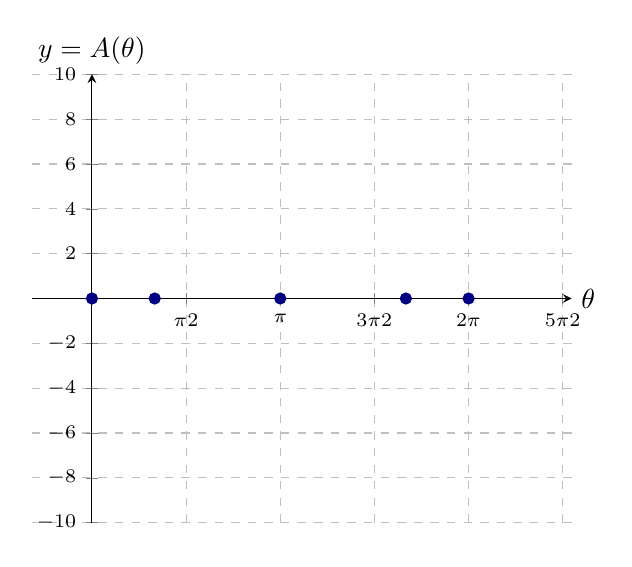
\begin{tikzpicture}
  \begin{axis}[
            domain=-1:8, ymax=10, xmax=8, ymin=-10, xmin=-1,
            axis lines =center, xlabel={$\theta$}, ylabel={$y = A(\theta)$}, grid = major, grid style={dashed},
            ytick={-10,-8,-6,-4,-2,2,4,6,8,10},
            xtick={-7.85, -6.28, -4.71, -3.14, -1.57, 0, 1.57, 3.142, 4.71, 6.28, 7.85},
            xticklabels={$\tfrac{-5\pi}{2}$,$-2\pi$,$\tfrac{-3\pi}{2}$,$-\pi$, $\tfrac{-\pi}{2}$, $0$, $\tfrac{\pi}{2}$, $\pi$, $\tfrac{3\pi}{2}$, $2\pi$, $\tfrac{5\pi}{2}$},
            yticklabels={$-10$,$-8$,$-6$,$-4$,$-2$,$2$,$4$,$6$,$8$,$10$}, 
            ticklabel style={font=\scriptsize},
            every axis y label/.style={at=(current axis.above origin),anchor=south},
            every axis x label/.style={at=(current axis.right of origin),anchor=west},
            axis on top
          ]
          
            \addplot[color=penColor,fill=penColor,only marks,mark=*] coordinates{(0,0)};
            \addplot[color=penColor,fill=penColor,only marks,mark=*] coordinates{(1.047,0)};
            \addplot[color=penColor,fill=penColor,only marks,mark=*] coordinates{(3.141,0)};
            \addplot[color=penColor,fill=penColor,only marks,mark=*] coordinates{(5.236,0)};
            \addplot[color=penColor,fill=penColor,only marks,mark=*] coordinates{(6.282,0)};


  \end{axis}
\end{tikzpicture}
\end{image}




The function is continuous. Therefore, the function either changes sign across each zero or it maintains its sign. The graph either crosses the axis at the intercepts or the graph bounces back and maintains its sign.


We can follow the sign of $A$ through its factors.

\[   A(\theta) = \sin(\theta) (1 - 2\cos(\theta))   \]



\begin{explanation}

$\blacktriangleright$  Across $0$, $\sin(\theta)$ changes sign. It goes from negative to positive. On the other hand $1 - 2\cos(\theta)$ stays negative on either side of $0$.  Therefore, $A(\theta)$ changes sign.  It goes from positive to negative and the graph crosses the axis at $(0, 0)$.

$\blacktriangleright$  Across $\frac{\pi}{3}$, $\sin(\theta)$ remains positive. However, $1 - 2\cos(\theta)$ changes sign.  It goes from negative to positive. Therefore, $A(\theta)$ changes sign. It changes from negative to positive and the graph crosses the axis at $\left( \frac{\pi}{3}, 0 \right)$.


$\blacktriangleright$  Across $\pi$, $\sin(\theta)$ changes sign, from positive to negative.  $1 - 2\cos(\theta)$ stays positive on either side of $\pi$.  Therefore, $A(\theta)$ changes sign from positive to negative and the graph crosses the axis at $(\pi, 0)$.


$\blacktriangleright$  Across $\frac{5\pi}{3}$, $\sin(\theta)$ remains negative. However, $1 - 2\cos(\theta)$ changes sign.  It goes from positive to negative. Therefore, $A(\theta)$ changes sign. It changes from negative to positive and the graph crosses the axis at $\left( \frac{5\pi}{3}, 0 \right)$.



\end{explanation}






The behavior at $2\pi$ is the same as the behavior at $0$, since $A$ is periodic. \\





We now know that $A(t)$ is negative when $t$ is slightly positive and that $A$ changes signs at each zero. We can sketch a rough idea of how the graph moves.










\begin{image}
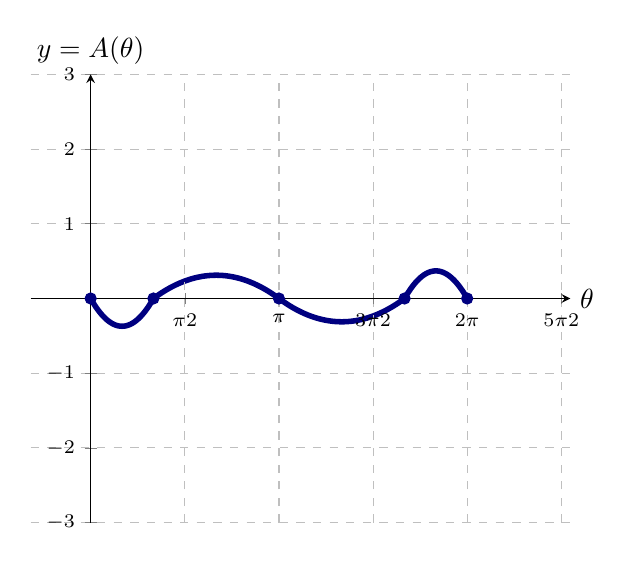
\begin{tikzpicture}
  \begin{axis}[
            domain=-1:8, ymax=3, xmax=8, ymin=-3, xmin=-1,
            axis lines =center, xlabel={$\theta$}, ylabel={$y = A(\theta)$}, grid = major, grid style={dashed},
            ytick={-3,-2,-1,1,2,3},
            xtick={1.57, 3.142, 4.71, 6.28, 7.85},
            xticklabels={$\tfrac{\pi}{2}$, $\pi$, $\tfrac{3\pi}{2}$, $2\pi$, $\tfrac{5\pi}{2}$},
            yticklabels={$-3$,$-2$,$-1$,$1$,$2$,$3$}, 
            ticklabel style={font=\scriptsize},
            every axis y label/.style={at=(current axis.above origin),anchor=south},
            every axis x label/.style={at=(current axis.right of origin),anchor=west},
            axis on top
          ]
          



            \addplot[color=penColor,fill=penColor,only marks,mark=*] coordinates{(0,0)};
            \addplot[color=penColor,fill=penColor,only marks,mark=*] coordinates{(1.047,0)};
             \addplot[color=penColor,fill=penColor,only marks,mark=*] coordinates{(3.14,0)};
            \addplot[color=penColor,fill=penColor,only marks,mark=*] coordinates{(5.236,0)};
            \addplot[color=penColor,fill=penColor,only marks,mark=*] coordinates{(6.28,0)};


            \addplot [line width=2, penColor, smooth,samples=300,domain=(0:1.047)] {1.355*(x)*(x-1.047)};
            \addplot [line width=2, penColor, smooth,samples=300,domain=(1.047:3.141)] {-0.284*(x-1.047)*(x-3.141)};
            \addplot [line width=2, penColor, smooth,samples=300,domain=(3.141:5.236)] {0.284*(x-3.141)*(x-5.236)};
            \addplot [line width=2, penColor, smooth,samples=300,domain=(5.236:6.28)] {-1.355*(x-5.236)*(x-6.28)};






  \end{axis}
\end{tikzpicture}
\end{image}

































$\blacktriangleright$  The range is difficult to determine from here.  It depends on how high and low the maximum and minimum are.  

We do know that $\sin(\theta)$ and $\cos(\theta)$ can't get greater than $1$ or less than $-1$.  That tells us that $1 -2\cos(\theta)$ can't get greater than $3$.   So, the range must be inside $[-3, 3]$.





A better graph seems to agree with this reasoning.





\begin{image}
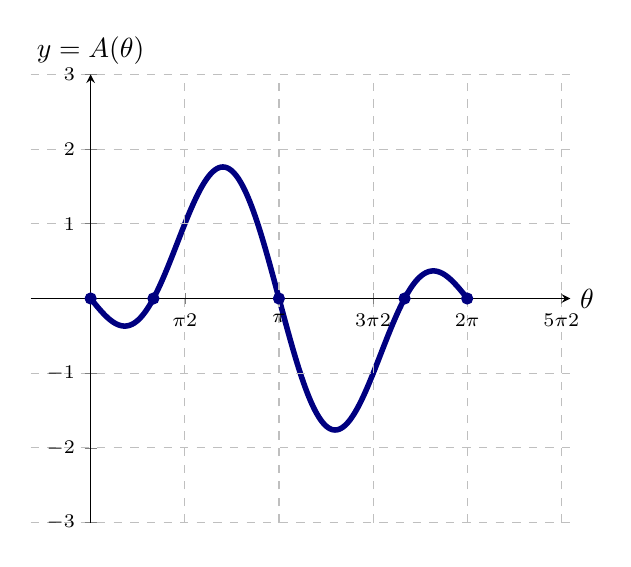
\begin{tikzpicture}
  \begin{axis}[
            domain=-1:8, ymax=3, xmax=8, ymin=-3, xmin=-1,
            axis lines =center, xlabel={$\theta$}, ylabel={$y = A(\theta)$}, grid = major, grid style={dashed},
            ytick={-3,-2,-1,1,2,3},
            xtick={1.57, 3.142, 4.71, 6.28, 7.85},
            xticklabels={$\tfrac{\pi}{2}$, $\pi$, $\tfrac{3\pi}{2}$, $2\pi$, $\tfrac{5\pi}{2}$},
            yticklabels={$-3$,$-2$,$-1$,$1$,$2$,$3$}, 
            ticklabel style={font=\scriptsize},
            every axis y label/.style={at=(current axis.above origin),anchor=south},
            every axis x label/.style={at=(current axis.right of origin),anchor=west},
            axis on top
          ]
          



            \addplot[color=penColor,fill=penColor,only marks,mark=*] coordinates{(0,0)};
            \addplot[color=penColor,fill=penColor,only marks,mark=*] coordinates{(1.047,0)};
             \addplot[color=penColor,fill=penColor,only marks,mark=*] coordinates{(3.14,0)};
            \addplot[color=penColor,fill=penColor,only marks,mark=*] coordinates{(5.236,0)};
            \addplot[color=penColor,fill=penColor,only marks,mark=*] coordinates{(6.28,0)};


            \addplot [line width=2, penColor, smooth,samples=300,domain=(0:6.28)] {sin(deg(x))-sin(deg(2*x))};





  \end{axis}
\end{tikzpicture}
\end{image}



The graph suggests a lot to us (which is why we like graphs).  The graph gives us reason to believe that the range is inside the interval $[-2, 2]$.  However, we'll need Calculus to get exact values for the maximum and minimum values.


























The graph suggests a lot to us (which is why we like graphs).  The graph also suggests that there are critical numbers in between the zeros.  







$\blacktriangleright$ maximums and minimums

\begin{itemize}
\item $A$ has a critical number between $\frac{2\pi}{3}$ and $\pi$, which corresponds to a global (and local) maximum.
\item $A$ has a critical number between $\pi$ and $\frac{5\pi}{3}$, which corresponds to a global (and local) minimum.
\item $A$ has a critical number between $\frac{5\pi}{3}$ and $2\pi$, which corresponds to a local maximum.
\item $A$ has a critical number between $0$ and $\frac{2\pi}{3}$, which corresponds to a local minimum.
\end{itemize}


Let's call these critical numbers $c_1$, $c_2$, $c_3$, and $c_4$.













\begin{image}
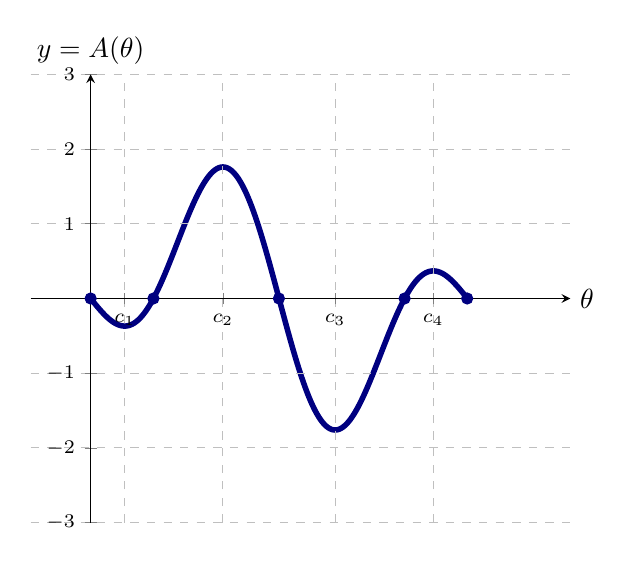
\begin{tikzpicture}
  \begin{axis}[
            domain=-1:8, ymax=3, xmax=8, ymin=-3, xmin=-1,
            axis lines =center, xlabel={$\theta$}, ylabel={$y = A(\theta)$}, grid = major, grid style={dashed},
            ytick={-3,-2,-1,1,2,3},
            xtick={0.568, 2.206, 4.078, 5.715},
            xticklabels={$c_1$, $c_2$, $c_3$, $c_4$},
            yticklabels={$-3$,$-2$,$-1$,$1$,$2$,$3$}, 
            ticklabel style={font=\scriptsize},
            every axis y label/.style={at=(current axis.above origin),anchor=south},
            every axis x label/.style={at=(current axis.right of origin),anchor=west},
            axis on top
          ]
          



            \addplot[color=penColor,fill=penColor,only marks,mark=*] coordinates{(0,0)};
            \addplot[color=penColor,fill=penColor,only marks,mark=*] coordinates{(1.047,0)};
             \addplot[color=penColor,fill=penColor,only marks,mark=*] coordinates{(3.14,0)};
            \addplot[color=penColor,fill=penColor,only marks,mark=*] coordinates{(5.236,0)};
            \addplot[color=penColor,fill=penColor,only marks,mark=*] coordinates{(6.28,0)};


            \addplot [line width=2, penColor, smooth,samples=300,domain=(0:6.28)] {sin(deg(x))-sin(deg(2*x))};





  \end{axis}
\end{tikzpicture}
\end{image}
















$\blacktriangleright$ Rate-of-Change

\begin{itemize}
\item $A$ is decreasing on $[0, c_1]$.
\item $A$ is increasing on $[c_1, c_2]$.
\item $A$ is decreasing on $[c_2, c_3]$.
\item $A$ is increasing on $[c_3, c_4]$.
\item $A$ is decreasing on $[c_4, 2\pi]$.
\end{itemize}


Of course, we could use the graph to approximate values for these critical numbers.




\section*{with Calculus}

Calculus will give us the tools to discover a formula for the derivative of $A$.


\[   A'(\theta) = \cos(\theta)-2 \cos(2\theta)    \]


The critical numbers would be where $A'(\theta) = 0$.



\begin{align*}
0    & = \cos(\theta)-2 \cos(2\theta)   \\
     & = \cos(\theta) - 2 (2 \cos^2(\theta) - 1)    \\
     & = -4 \cos^2(\theta) + \cos(\theta) + 2   \\
     & = 4 \cos^2(\theta) - \cos(\theta) - 2   \\
\end{align*}


We have a quadratic equation.  It doesn't factor nicely, so we'll go with the quadratic formula.



\[   \cos(\theta) = \frac{1 \pm \sqrt{1 - 4 (4)(-2)}}{2 \cdot 4}  = \frac{1 \pm \sqrt{33}}{8}        \]




Let's take each of these separately.



$\blacktriangleright$  $\cos(\theta) = \frac{1 + \sqrt{33}}{8}   \approx  0.843$


We are looking for an angle whose cosine is $\frac{1 + \sqrt{33}}{8}$.  This is positive, therefore, there are two such angles. One in the first quadrant.  That would be $\arccos\left(\frac{1 + \sqrt{33}}{8}\right)$




\begin{image}
\begin{tikzpicture}
  \begin{axis}[
            xmin=-1.1,xmax=1.1,ymin=-1.1,ymax=1.1,
            axis lines=center,
            width=4in,
            xtick={-1,1},
            ytick={-1,1},
            clip=false,
            unit vector ratio*=1 1 1,
            xlabel=$x$, ylabel=$y$,
            every axis y label/.style={at=(current axis.above origin),anchor=south},
            every axis x label/.style={at=(current axis.right of origin),anchor=west},
          ]        
          \addplot [dashed, smooth, domain=(0:360)] ({cos(x)},{sin(x)}); %% unit circle

          \addplot [textColor] plot coordinates {(0,0) (0.843,0.538)}; %% 40 degrees

          %\addplot [ultra thick,penColor] plot coordinates {(.766,0) (.766,.643)}; %% 40 degrees
          %\addplot [ultra thick,penColor2] plot coordinates {(0,0) (.766,0)}; %% 40 degrees
          
          %\addplot [ultra thick,penColor3] plot coordinates {(1,0) (1,.839)}; %% 40 degrees          

          \addplot [textColor,smooth, domain=(0:32.53)] ({.15*cos(x)},{.15*sin(x)});
          %\addplot [very thick,penColor] plot coordinates {(0,0) (.766,.643)}; %% sector
          %\addplot [very thick,penColor] plot coordinates {(0,0) (1,0)}; %% sector
          %\addplot [very thick, penColor, smooth, domain=(0:40)] ({cos(x)},{sin(x)}); %% sector
          \node at (axis cs:.15,0.07) [anchor=west] {$c_1$};
          %\node[penColor, rotate=-90] at (axis cs:.84,.322) {$\sin(\theta)$};
          %\node[penColor2] at (axis cs:.383,0) [anchor=north] {$\cos(\theta)$};
          %\node[penColor3, rotate=-90] at (axis cs:1.06,.322) {$\tan(\theta)$};
        \end{axis}
\end{tikzpicture}
\end{image}




There is a second angle in the fourth quadrant where cosine is $\frac{1 + \sqrt{33}}{8}$.  This angle could be described as $-\arccos\left(\frac{1 + \sqrt{33}}{8}\right)$.  However, our chosen interval to examine is $[0, 2\pi)$. So, the angle in the fourth quadrant is $2\pi - \arccos\left(\frac{1 + \sqrt{33}}{8}\right)$







\begin{image}
\begin{tikzpicture}
  \begin{axis}[
            xmin=-1.1,xmax=1.1,ymin=-1.1,ymax=1.1,
            axis lines=center,
            width=4in,
            xtick={-1,1},
            ytick={-1,1},
            clip=false,
            unit vector ratio*=1 1 1,
            xlabel=$x$, ylabel=$y$,
            every axis y label/.style={at=(current axis.above origin),anchor=south},
            every axis x label/.style={at=(current axis.right of origin),anchor=west},
          ]        
          \addplot [dashed, smooth, domain=(0:360)] ({cos(x)},{sin(x)}); %% unit circle

          \addplot [textColor] plot coordinates {(0,0) (0.843,0.538)}; %%
          \addplot [textColor] plot coordinates {(0,0) (0.843,-0.538)};

          %\addplot [ultra thick,penColor] plot coordinates {(.766,0) (.766,.643)}; %% 40 degrees
          %\addplot [ultra thick,penColor2] plot coordinates {(0,0) (.766,0)}; %% 40 degrees
          
          %\addplot [ultra thick,penColor3] plot coordinates {(1,0) (1,.839)}; %% 40 degrees          

          \addplot [textColor,smooth, domain=(0:32.53)] ({.15*cos(x)},{.15*sin(x)});
          \addplot [textColor,smooth, domain=(0:327.47)] ({.18*cos(x)},{.18*sin(x)});
          %\addplot [very thick,penColor] plot coordinates {(0,0) (.766,.643)}; %% sector
          %\addplot [very thick,penColor] plot coordinates {(0,0) (1,0)}; %% sector
          %\addplot [very thick, penColor, smooth, domain=(0:40)] ({cos(x)},{sin(x)}); %% sector
          \node at (axis cs:0.15,0.07) [anchor=west] {$c_1$};
          \node at (axis cs:-0.07,-0.20) [anchor=east] {$c_4$};
          %\node[penColor, rotate=-90] at (axis cs:.84,.322) {$\sin(\theta)$};
          %\node[penColor2] at (axis cs:.383,0) [anchor=north] {$\cos(\theta)$};
          %\node[penColor3, rotate=-90] at (axis cs:1.06,.322) {$\tan(\theta)$};
        \end{axis}
\end{tikzpicture}
\end{image}












$\blacktriangleright$  $\cos(\theta) = \frac{1 - \sqrt{33}}{8}   \approx  -0.593$


We are looking for an angle whose cosine is $\frac{1 - \sqrt{33}}{8}$.  This is negative, therefore, there are two such angles. One in the second quadrant.  That would be $\arccos\left(\frac{1 - \sqrt{33}}{8}\right)$




\begin{image}
\begin{tikzpicture}
  \begin{axis}[
            xmin=-1.1,xmax=1.1,ymin=-1.1,ymax=1.1,
            axis lines=center,
            width=4in,
            xtick={-1,1},
            ytick={-1,1},
            clip=false,
            unit vector ratio*=1 1 1,
            xlabel=$x$, ylabel=$y$,
            every axis y label/.style={at=(current axis.above origin),anchor=south},
            every axis x label/.style={at=(current axis.right of origin),anchor=west},
          ]        
          \addplot [dashed, smooth, domain=(0:360)] ({cos(x)},{sin(x)}); %% unit circle

          \addplot [textColor] plot coordinates {(0,0) (-0.593,0.8052)}; %% 40 degrees

          %\addplot [ultra thick,penColor] plot coordinates {(.766,0) (.766,.643)}; %% 40 degrees
          %\addplot [ultra thick,penColor2] plot coordinates {(0,0) (.766,0)}; %% 40 degrees
          
          %\addplot [ultra thick,penColor3] plot coordinates {(1,0) (1,.839)}; %% 40 degrees          

          \addplot [textColor,smooth, domain=(0:126.37)] ({.18*cos(x)},{.18*sin(x)});
          %\addplot [very thick,penColor] plot coordinates {(0,0) (.766,.643)}; %% sector
          %\addplot [very thick,penColor] plot coordinates {(0,0) (1,0)}; %% sector
          %\addplot [very thick, penColor, smooth, domain=(0:40)] ({cos(x)},{sin(x)}); %% sector
          \node at (axis cs:0.14,0.2) [anchor=south] {$c_2$};
          %\node[penColor, rotate=-90] at (axis cs:.84,.322) {$\sin(\theta)$};
          %\node[penColor2] at (axis cs:.383,0) [anchor=north] {$\cos(\theta)$};
          %\node[penColor3, rotate=-90] at (axis cs:1.06,.322) {$\tan(\theta)$};
        \end{axis}
\end{tikzpicture}
\end{image}




There is a fourth angle in the third quadrant where cosine is $\frac{1 - \sqrt{33}}{8}$.  This third quadrant angle has the same reference angle as $c_2$. Therefore, $c_3 = 2\pi - \arccos\left(\frac{1 - \sqrt{33}}{8}\right)$.






\begin{image}
\begin{tikzpicture}
  \begin{axis}[
            xmin=-1.1,xmax=1.1,ymin=-1.1,ymax=1.1,
            axis lines=center,
            width=4in,
            xtick={-1,1},
            ytick={-1,1},
            clip=false,
            unit vector ratio*=1 1 1,
            xlabel=$x$, ylabel=$y$,
            every axis y label/.style={at=(current axis.above origin),anchor=south},
            every axis x label/.style={at=(current axis.right of origin),anchor=west},
          ]        
          \addplot [dashed, smooth, domain=(0:360)] ({cos(x)},{sin(x)}); %% unit circle

          \addplot [textColor] plot coordinates {(0,0) (-0.593,0.8052)}; %% 40 degrees
          \addplot [textColor] plot coordinates {(0,0) (-0.593,-0.8052)};

          %\addplot [ultra thick,penColor] plot coordinates {(.766,0) (.766,.643)}; %% 40 degrees
          %\addplot [ultra thick,penColor2] plot coordinates {(0,0) (.766,0)}; %% 40 degrees
          
          %\addplot [ultra thick,penColor3] plot coordinates {(1,0) (1,.839)}; %% 40 degrees          

          \addplot [textColor,smooth, domain=(0:126.37)] ({.18*cos(x)},{.18*sin(x)});
          \addplot [textColor,smooth, domain=(0:233.63)] ({.14*cos(x)},{.14*sin(x)});
          %\addplot [very thick,penColor] plot coordinates {(0,0) (.766,.643)}; %% sector
          %\addplot [very thick,penColor] plot coordinates {(0,0) (1,0)}; %% sector
          %\addplot [very thick, penColor, smooth, domain=(0:40)] ({cos(x)},{sin(x)}); %% sector
          \node at (axis cs:0.14,0.2) [anchor=south] {$c_2$};
          \node at (axis cs:-0.24,-0.2) [anchor=south] {$c_3$};
          %\node[penColor, rotate=-90] at (axis cs:.84,.322) {$\sin(\theta)$};
          %\node[penColor2] at (axis cs:.383,0) [anchor=north] {$\cos(\theta)$};
          %\node[penColor3, rotate=-90] at (axis cs:1.06,.322) {$\tan(\theta)$};
        \end{axis}
\end{tikzpicture}
\end{image}




We want exact answers, when possible, and we have exact answers with Calculus.

For us, without the derivative, we could approximate the critical numbers from a graph as well as the extreme values of $A$.



\begin{center}
\desmos{waae40vtar}{400}{300}
\end{center}




\begin{itemize}
  \item $c_1 \approx 0.568$
  \item $c_2 \approx 2.206$
  \item $c_3 \approx 4.078$
  \item $c_4 \approx 5.715$
\end{itemize}







$\blacktriangleright$ \textbf{Extrema}




$\rhd$ We have a global maximum of $A(c_2)$:


\[  A(c_2) = \sin\left(\arccos\left(\frac{1 - \sqrt{33}}{8}\right)\right) - \sin\left(2 \arccos\left(\frac{1 - \sqrt{33}}{8}\right)\right) \approx 1.76   \]




at $c_2 = \arccos\left(\frac{1 - \sqrt{33}}{8}\right) \approx 2.206$. \\









$\rhd$ We have a global minimum of $A(c_3)$:


\[  A(c_3) = \sin\left(   2\pi - \arccos\left(\frac{1 - \sqrt{33}}{8}\right)    \right) - \sin\left(2  \left(     2\pi - \arccos\left(\frac{1 - \sqrt{33}}{8}\right)     \right) \right)  \approx -1.76  \]




at $c_3 = 2\pi - \arccos\left(\frac{1 - \sqrt{33}}{8}\right) \approx 4.078$. \\








$\rhd$ We have a local minimum of $A(c_1)$:


\[  A(c_1) = \sin\left(   \arccos\left(\frac{1 + \sqrt{33}}{8}\right)    \right) - \sin\left(2  \arccos\left(\frac{1 + \sqrt{33}}{8}\right)   \right)  \approx -0.369  \]




at $c_1 = \arccos\left(\frac{1 + \sqrt{33}}{8}\right) \approx 0.568$.   \\












$\rhd$ We have a local maximum of $A(c_4)$:


\[  A(c_4) = \sin\left(   2\pi - \arccos\left(\frac{1 + \sqrt{33}}{8}\right)   \right) - \sin\left(2  (2\pi - \arccos\left(\frac{1 + \sqrt{33}}{8}\right))  \right)  \approx 0.369  \]




at $c_4 = 2\pi - \arccos\left(\frac{1 + \sqrt{33}}{8}\right) \approx 5.715$.   \\














$\blacktriangleright$ Rate-of-Change

\begin{itemize}
\item $A$ is decreasing on approximately $[0, 0.568]$.
\item $A$ is increasing on approximately $[0.568, 2.206]$.
\item $A$ is decreasing on approximately $[2.206, 4.078]$.
\item $A$ is increasing on approximately $[4.078, 5.715]$.
\item $A$ is decreasing on approximately $[5.715, 2\pi]$.
\end{itemize}








\begin{center}
\textbf{\textcolor{green!50!black}{ooooo-=-=-=-ooOoo-=-=-=-ooooo}} \\

more examples can be found by following this link\\ \link[More Examples of More Function Analysis]{https://ximera.osu.edu/csccmathematics/precalculus2/precalculus2/moreFunctionAnalysis/examples/exampleList}

\end{center}




\end{document}
